% Created 2016-08-17 Wed 14:38
\documentclass[tikz]{standalone}

\usepackage[utf8]{inputenc}
\usepackage[T1]{fontenc}

\usepackage{circledsteps}

\RequirePackage{xcolor}

%% HPI color definitions according to the design manual
% These do not exactly match the RGB values used in the Powerpoint slide master due to unknown reasons
\definecolor{hpiyellow}{RGB}{246,168,0}
\definecolor{hpiorange}{RGB}{221,97,8}
\definecolor{hpired}{RGB}{177,6,58}
\definecolor{hpigray}{RGB}{90,96,101}
\definecolor{hpiblue}{RGB}{0,122,158}


\renewcommand{\sfdefault}{neosans}
% Different font weights for neosans
\newcommand{\textl}[1]{{\fontseries{l}\selectfont #1}} % light
\newcommand{\textm}[1]{{\fontseries{m}\selectfont #1}} % medium, same as default weight
\newcommand{\textsb}[1]{{\fontseries{sb}\selectfont #1}} % semibold
\newcommand{\textmb}[1]{{\fontseries{mb}\selectfont #1}} % bold, same as \textbf
\newcommand{\texteb}[1]{{\fontseries{eb}\selectfont #1}} % extra bold
\newcommand{\textub}[1]{{\fontseries{ub}\selectfont #1}} % ultra bold

\tikzset{every picture/.style={/utils/exec={\sffamily}}}
\tikzset{flipflop RSflanke/.style={
  flipflop,
  flipflop def={t1=S, t2=C, c2=1, t3=R, t6=Q, t4={\ctikztextnot{Q}}}
}}


\tikzset{
  mechanicalSwitch/.pic={
    \coordinate (-inUp) at (135:2); 
    \coordinate (-inDown) at (235:2);
    \coordinate (-out) at (2,0);
    \coordinate (-center) at (0,0);
    
    \draw (0,0) circle [radius = 2cm];
    \draw [fill=gray!20] (0,0) circle [radius = 0.2cm];

    \draw (0, 0) -- (2, 0);
    \draw (135:.8) -- (135:2); 
    \draw (225:.8) -- (225:2); 

    \draw [fill=gray!20] (2, 0) circle [radius=0.05cm]; 
    \draw [fill=gray!20] (135:2) circle [radius=0.05cm]; 
    \draw [fill=gray!20] (225:2) circle [radius=0.05cm]; 

    
    \draw [thick] (0,0) -- (175:1.5); 

    \draw [dashed, <->, domain=135:225] plot ({cos(\x)}, {sin(\x)}); 
  },
  mechanicalSwitchClosed/.pic={
    \coordinate (-inUp) at (135:2); 
    \coordinate (-inDown) at (255:2);
    \coordinate (-out) at (2,0);
    \coordinate (-center) at (0,0);
    \draw (0,0) circle [radius = 2cm];
    \draw [fill=gray!20] (0,0) circle [radius = 0.2cm];

    \draw (0, 0) -- (2, 0);
    \draw (135:.8) -- (135:2); 
    \draw (225:.8) -- (225:2); 

    \draw [fill=gray!20] (2, 0) circle [radius=0.05cm]; 
    \draw [fill=gray!20] (135:2) circle [radius=0.05cm]; 
    \draw [fill=gray!20] (225:2) circle [radius=0.05cm]; 

    
    \draw [thick] (0,0) -- (135:2); 

    \draw [dashed, <->, domain=135:225] plot ({cos(\x)}, {sin(\x)}); 
  }
}


\usetikzlibrary{calc}
\usetikzlibrary{positioning}


\usepackage{amsmath}
\usetikzlibrary{ext.positioning-plus,backgrounds,fit,shapes.geometric}

\begin{document}


% \begin{tikzpicture}[every fit/.style={rectangle,rounded corners,inner sep=2pt}]
\begin{tikzpicture}[every fit/.style={ellipse,inner sep=0pt}]

  \label{page:routing:hierarchy:full}
  
  %   blue group

  \begin{scope}[every node/.style={draw=hpiblue,fill=hpiblue!50,circle},
    ]
    \foreach \x/\y [count=\i] in {0/0,2/-1,2.5/-2,3/0.5} {
      \node (a\i) at (\x,\y) {$A_\i$}; 
    }

    \scoped[on background layer] \node [fit=(a1)(a2)(a3)(a4),draw=hpiblue,fill=hpiblue!10] (a) {};

  \foreach \n/\m in {1/2,2/3,2/4,3/4} {
    \draw (a\n) -- (a\m); 
  }
  
  \end{scope}

  \begin{scope}[every node/.style={fill=hpiorange!60,circle},xshift=8cm]

    \foreach \x/\y [count=\i] in {0/0,1.25/0,2/1,2.5/-1} {
      \node (b\i) at (\x,\y) {$B_\i$}; }

    % \node (b1) at (0,0) {}; 
    % \node (b2) at (1,0) {}; 
    % \node (b3) at (2,1) {}; 
    % \node (b4) at (2.5,-1) {}; 

    \scoped[on background layer] \node [fit=(b1)(b2)(b3)(b4),draw=hpiorange,fill=hpiorange!10] (b) {}; 

    \foreach \n/\m in {1/2,2/3,2/4,3/4,1/3,1/4} {
      \draw (b\n) -- (b\m); }

  \end{scope}

  \begin{scope}[every node/.style={fill=hpiyellow!60,circle},yshift=-6cm]

    \foreach \x/\y [count=\i] in {-1/-1,0/0,1/0,0.75/-1,2/-1.25,2.5/-0.25} {
      \node (c\i) at (\x,\y) {$C_\i$}; }

    % \node (c1) at (0,0) {}; 
    % \node (c2) at (0.5,0.5) {}; 
    % \node (c3) at (1,0) {}; 
    % \node (c4) at (0.75,-1) {}; 
    % \node (c5) at (2,-1.25) {}; 
    % \node (c6) at (2.5,-0.25) {}; 

    \scoped[on background layer] \node [fit=(c1)(c2)(c3)(c4)(c5)(c6),draw=hpiyellow,fill=hpiyellow!10] (b) {}; 


    \foreach \n/\m in {1/2,2/3,1/3,3/4,3/6,4/6,5/6} {
      \draw (c\n) -- (c\m); }

  \end{scope}

  \begin{scope}[every node/.style={fill=hpired!60,circle},yshift=-6cm,xshift=8cm]

    \foreach \x/\y [count=\i] in {0/0,1/0,0.25/2,0.25/-1.5,1.25/1.25} {
      \node (d\i) at (\x,\y) {$D_\i$}; }

    % \node (d1) at (0,0) {}; 
    % \node (d2) at (1,0) {}; 
    % \node (d3) at (0.25,2) {}; 
    % \node (d4) at (0.25,-1.5) {}; 
    % \node (d5) at (0.5,1.25) {}; 

    \scoped[on background layer] \node [fit=(d1)(d2)(d3)(d4)(d5),draw=hpired,fill=hpired!10] (b) {}; 

    \foreach \n/\m in {1/2,1/3,2/5,2/4,1/4,3/5} {
      \draw (d\n) -- (d\m); }

  \end{scope}


    \foreach \n/\m in {a1/c2,a4/b1,b4/d3,d1/c6} {
      \draw (\n) -- (\m); }


  
\end{tikzpicture}

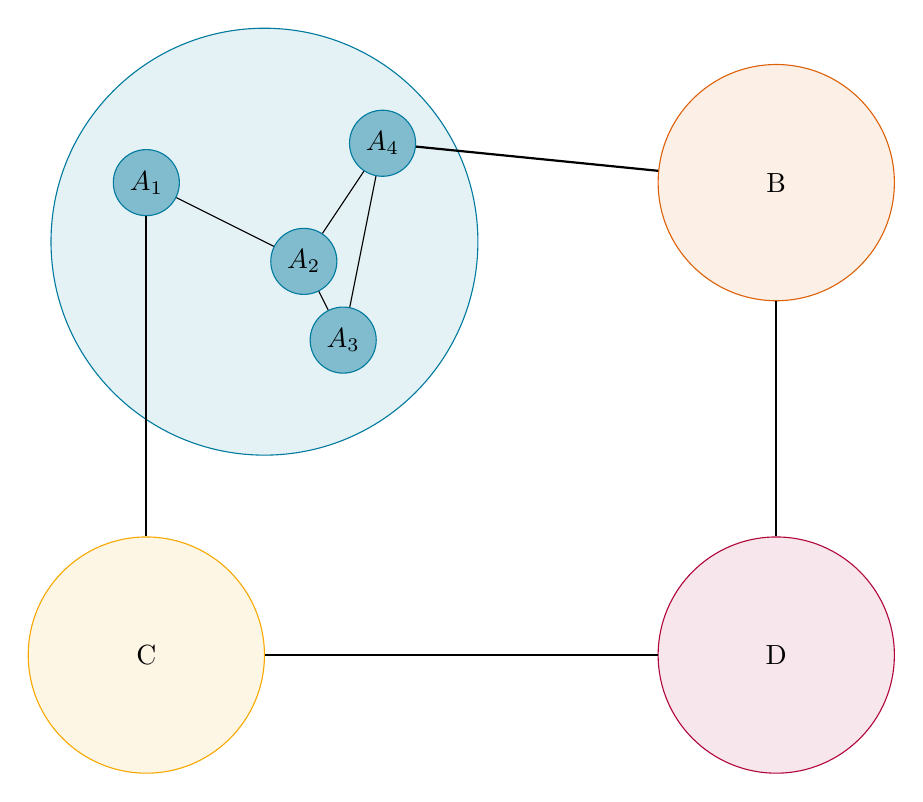
\begin{tikzpicture}
  \label{page:routing:hierarchy:limited}

  
  \begin{scope}[every node/.style={draw=hpiblue,fill=hpiblue!50,circle},
    ]
    \foreach \x/\y [count=\i] in {0/0,2/-1,2.5/-2,3/0.5} {
      \node (a\i) at (\x,\y) {$A_\i$}; 
    }

    \scoped[on background layer] \node [fit=(a1)(a2)(a3)(a4),draw=hpiblue,fill=hpiblue!10] (a) {};

  \foreach \n/\m in {1/2,2/3,2/4,3/4} {
    \draw (a\n) -- (a\m); 
  }
  
  \end{scope}

  \node [fill=hpiorange!10, draw=hpiorange, circle, minimum width=3cm] at (8,0)  (b) {B}; 
  \node [fill=hpiyellow!10, draw=hpiyellow, circle, minimum width=3cm] at (0,-6) (c) {C}; 
  \node [fill=hpired!10, draw=hpired, circle, minimum width=3cm] at (8,-6) (d) {D};

  \draw [thick] (a1) -- (c); 
  \draw [thick] (a4) -- (b);
  \draw [thick] (b) -- (d) -- (c); 
\end{tikzpicture}

\end{document} 